%!TEX ROOT=formularioFisica.tex

\section{Elettrostatica}\label{sec:elettrostatica}
L'Elettrostatica studia le cariche elettriche nei corpi e come reagiscono fra di loro.\\
Un concetto fondamentale � quello di \textbf{carica}. La carica (identificata con $Q$) � determinata 
dalla somma di tutte le cariche degli elettroni all'interno di ogni corpo. La sua unit� di misura � il 
\emph{Coulomb} ($C$).\\[\baselineskip]
Si noti che nelle seguenti formule, $\varepsilon$ � definito come 
$\varepsilon = \varepsilon_0\varepsilon_r$ dove $\varepsilon_0$ � \hyperref[tab:e0]{la costante
dielettrica nel vuoto} e $\varepsilon_r$ � la costante dielettrica nel mezzo (nel vuoto � $0$).\\
Per gli esercizi si vada a pagina~\pageref{ex:elettrostatica}.

\subsection{Legge di Coulomb}
Attraverso la legge di Coulomb (da non essere confusa con il teorema di Coulomb) si trova la forza che 
intercorre tra due corpi carichi. Si noti che questa formula pu� essere usata solo se i corpi sono 
puntiformi e fermi.
\begin{equation*}
F = k_0\frac{Q_1Q_2}{r^2} = \frac{1}{4\pi\varepsilon}\frac{Q_1Q_2}{r^2}
\end{equation*}
\hyperref[tab:k0]{$k_0$}: $9.11\cdot10^9\,\text{N}\cdot\text{m}^2\text{/C}^2$

\subsection{Campo elettrico}
Il campo elettrico � generato da una carica. Esso � un campo vettoriale, ci� significa che ad ogni
suo punto si associa un vettore.\\ 
Il campo elettrico pu� essere uniforme, ovvero a tutti i punti si associa un vettore uguale.\\
Verranno ora riportate tutte le formule che permettono di trovare o il modulo o il vettore di un
campo elettrico.

\begin{alignat*}{2}
E &= k_0\frac{Q}{r^2} & &\text{Solo se puntiforme}\\
\vec{E} &= \frac{\vec{F}}{q} &\qquad \vec{E} &= \sum\limits_{i=0}^{n} \vec{E}_n\\
E &= -\frac{\Delta V}{\Delta x} & &
\end{alignat*}
%E &= \frac{\sigma}{2\varepsilon_0} & &\text{Se in un condensatore, si divida solo per } \varepsilon\\
%E &= -\frac{\Delta V}{\Delta x} & & \\
\hyperref[tab:k0]{$k_0$}: $9.11\cdot10^9\,\text{N}\cdot\text{m}^2\text{/C}^2$\\
$\Delta V$: d.d.p\\
$\Delta x$: distanza tra le superfici

\subsubsection{Campo di una superficie piana infinita}
\begin{center}
	\begin{tikzpicture}
		\draw[dashed] (0,0) -- ++(1,0);
		\draw (1,0) -- ++(2,0);
		\draw[dashed] (3,0) -- ++(1,0);
		\draw[-stealth] (2,0.5) -- ++(0,-0.45)
			node[pos=0.5, left]{$\vec{E}$};
		\draw[-stealth] (2,-0.5) -- ++(0,0.45)
			node[pos=0.5, left]{$\vec{E}$};
		\node at (1,0.5){$q < 0$};
		
		\draw[dashed] (0,-2) -- ++(1,0);
		\draw (1,-2) -- ++(2,0);
		\draw[dashed] (3,-2) -- ++(1,0);
		\draw[stealth-] (2,-1.5) -- ++(0,-0.45)
			node[pos=0.5, left]{$\vec{E}$};
		\draw[stealth-] (2,-2.5) -- ++(0,0.45)
			node[pos=0.5, left]{$\vec{E}$};
		\node at (1,-1.5){$q > 0$};
	\end{tikzpicture}
\end{center}
\begin{equation*}
E = \frac{\left\lvert\sigma\right\rvert}{2\epsilon_0}
\end{equation*}
$\sigma$: densit� di carica $\left(\frac{Q}{A}\right)$

\subsubsection{Campo elettrico all'interno di un condensatore}
\begin{center}
	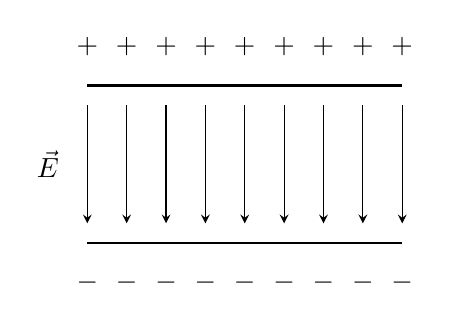
\begin{tikzpicture}
		\draw[thick] (0,0) -- ++(4,0);
		\foreach \ca in {0,0.5,1,...,4}{
			\node at (\ca,0.5){$+$};
			\node at (\ca,-2.5){$-$};
			\draw[-stealth] (\ca,-0.25) -- ++(0,-1.5);
		}
		\draw[thick] (0,-2) -- ++(4,0);
		\node at (-0.5,-1){$\vec{E}$};
	\end{tikzpicture}
\end{center}
\begin{equation*}
E = \frac{\sigma}{\varepsilon}
\end{equation*}
$\sigma$: densit� di carica $\left(\frac{Q}{A}\right)$

\subsection{Teorema di Coulomb}
Il teorema di Coulomb definisce il campo elettrico per una qualsiasi superficie.
\begin{equation*}
E = \frac{\sigma}{\epsilon_0}
\end{equation*}

\subsection{Flusso} \label{subsec:flusso}
Il flusso ($\Phi$) � la quantit� di campo elettrico ($\vec{E}$), che 
attraversa una superficie ($\vec{S}$).\\
Verranno ora riportate le formule per calcolare il flusso di una superficie.

\begin{alignat*}{2}
\Phi_i\left(\vec{E}\right) &= \vec{E}_i \cdot \vec{S_i} &\qquad &\\
\Phi_S\left(\vec{E}\right) &= \sum\limits_{i=0}^{n}\vec{E}_\cdot\vec{S_i} & &\\
\Phi_S\left(\vec{E}\right) &= E\cdot S\cos\theta & &\text{Se } S \text{ � piana e } E \text{ 
uniforme} 
\end{alignat*}

\subsection{Teorema di Gauss}
Il teorema di Gauss definisce il flusso di una superficie \emph{chiusa}.
\begin{equation*}
\Phi_{S_{CH}}\left(\vec{E}\right) = \frac{\sum\limits_{i=0}^{n}Q_i}{\varepsilon}
\end{equation*}

\subsection{Lavoro di un campo elettrico}
Quanto lavoro deve fare un campo elettrico per spostare una carica? Questa sottsezione � dedicata 
proprio a questo.

\begin{alignat*}{2}
L &= \Delta U &\qquad  &\text{Se riferito ad un campo elettrico}\\
L &= -\Delta U & &\text{Se riferito ad una carica}\\
L &= q\left[V_A - V_B\right] & &
\end{alignat*}

Al lavoro sono direttamente collegati \textbf{l'energia potenziale elettrica} ($U$) e 
\textbf{il potenziale elettrico} ($V$). Vengono ora riportate le formule per calcolarle.

\begin{alignat*}{2}
U &= k_0\frac{Q_1Q_2}{r} &\qquad V &= k_0\frac{Q}{r}
\end{alignat*}
\hyperref[tab:k0]{$k_0$}: $9.11\cdot10^9\,\text{N}\cdot\text{m}^2\text{/C}^2$

\subsubsection{Lavoro di una carica in un condensatore}
Il lavoro di una carica � equivalente all'energia interna.
\begin{equation*}
L = \frac{1}{2}qV = \frac{1}{2}CV^2 = \frac{1}{2}\frac{q^2}{C}
\end{equation*}

\subsection{Capacit� elettrica}
La capacit� elettrica indica quanta carica pu� immagazzinare un conduttore isolato. Verranno ora 
riportate le formule per calcolarla.

\begin{alignat*}{2}
C &= \frac{Q}{V} &\qquad &\\
C &= 4\pi\varepsilon & &\text{Specificamente in una sfera isolata}\\
C &= \frac{S\varepsilon}{d} & &\text{Specificamente in un condensatore piano}
\end{alignat*}
Nell'ultima formula, $d$ indica la distanza tra le due armature di un condensatore.

\subsection{Circuitazione}
La circuitazione ($C$) indica quanta carica passa per una linea chiusa ($\Gamma$).

\begin{equation*}
C_\Gamma\left(\vec{E}\right) = \sum\limits_{i=0}^{n}\vec{E}_i\cdot\vec{l}_i = 
\sum\limits_{i=0}^{n} E_i\cdot l_i\cos\theta
\end{equation*}
$l$: differenza di spostamento\\
Si noti che $theta$ � rispetto alla tangente, non alla normale come nel 
\hyperref[subsec:flusso]{Flusso}.

\subsection{Dielettrico all'interno di un condensatore}
Come cambia il campo elettrico all'interno di un condensatore se si inserisce un dielettrico?
\begin{equation*}
E_{RIS} = \frac{\sigma\cdot\sigma_p}{\varepsilon}
\end{equation*}

\subsection{Velocit� di deriva in un conduttore metallico}
� la velocit� media degli elettroni nel conduttore metallico.
\begin{equation*}
  v_d = \frac{i}{n\cdot A\cdot e}
\end{equation*}
\hyperref[tab:e-]{$e$}\\
$n$: numero di elettroni di conduzione\\
$A$: sezione del conduttore
$i$: carica massima

